\section{LLVM} \label{sec:2-llvm}

% TODO: update llvm information in references
\say{The LLVM Project is a collection of modular and reusable compiler and toolchain technologies. The LLVM project has multiple components. The core of the project is itself called “LLVM.” This project contains all of the tools, libraries, and header files needed to process intermediate representations and converts them into object files. Tools include an assembler, disassembler, bitcode analyzer, and bitcode optimizer.} \cite{llvm,lattner2004llvm}

\vspace{\baselineskip}

LLVM can be used as a compiler framework, separated into "front-end" and "back-end." The front-end contains the lexers and parsers, and it accepts the source code to a program and returns the \textbf{intermediate representation (IR)} of the program. The back-end converts the IR into machine language.

\vspace{\baselineskip}

For instrumentation, we insert the logging instructions into each basic block of the program in the front-end. \textbf{Clang} is part of the LLVM toolchain for compiling C/C++ source code. By definition, \say{\textbf{clang} is a C, C++, and Objective-C compiler that encompasses preprocessing, parsing, optimization, code generation, assembly, and linking.}\cite{clang} We extend the phases of compilation so that we are injecting the instructions in compilation. 

\vspace{\baselineskip}

LLVM converts an \textbf{IR} of a program into machine language instructions. The structure of the LLVM project is shown in Figure \ref{fig:llvm}:

\begin{figure}[htpb]
    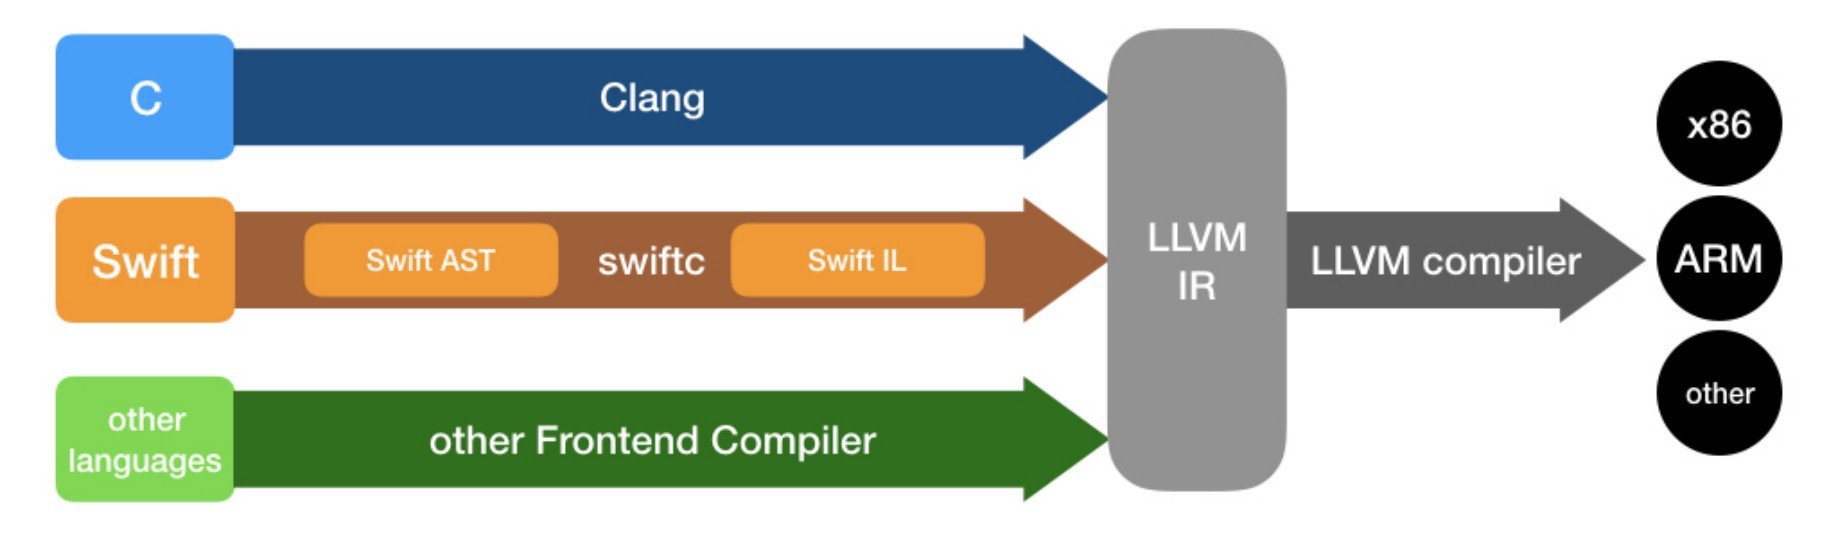
\includegraphics[width=\textwidth]{Chapter2/llvm.png}
    \centering
    \captionsetup{justification=centering}
    \caption{LLVM architecture: A front-end compiler generates the LLVM IR, and then it is converted into machine code \cite{omni_sci}}
    \label{fig:llvm}
\end{figure}

The instrumentation is applied before the IR generation, and the LLVM IR is fed into the LLVM compiler to generate the machine-specific instructions. As our instrumentation does not affect the LLVM IR compilation, we will not investigate the generated IR.


% Instrumentation
\subsection{Instrumentation and coverage measurements}
\label{instrumentation}

Waffle is based on AFL and we are extending the AFL's instrumentation in our work. The goal of using instrumentation for AFL is to differentiate code coverages. There are two techniques for instrumentation in AFL:

\begin{enumerate}
  \item \textit{$llvm\_mode$}: AFL takes the source code and an instrumentation recipe and generates the instrumented binary of the target program.
  \item \textit{$qemu\_mode$}: AFL leverages the QEMU mode to obtain instrumentation output for closed-source binaries. We don't use this mode in this thesis.
\end{enumerate}

In the LLVM recipe, we instantiate the bitmap and assign it to the shared memory for modifications. The remaining instructions for the recipe will be applied on the basic blocks in \textbf{AFLCoverage} module. This module takes effect in compilation of the program before the generation of IR. We can see some of the implementation of this \textbf{pass} in Listing \ref{lst:afl-llvm}:

\lstinputlisting[language=C++,style=CodeStyle,label={lst:afl-llvm},caption={AFLCoverage module}]{Codes/Chapter2/afl_llvm_pass.cpp}

The recipe for instrumentation fills out the coverage bitmap with the hash values of the paths executed. The instructions are as followed:

\begin{lstlisting}[language=C++,style=CodeStyle,label={lst:hash},caption={Select element and update in shared\_mem}]
  cur_location = <COMPILE_TIME_RANDOM>;
  shared_mem[cur_location ^ prev_location]++; 
  prev_location = cur_location >> 1;
\end{lstlisting}

AFL instruments by adding these instructions into basic blocks. First, a random value is assigned to \textit{curr\_location}. Next, it is XORed with the previous location's value, \textit{prev\_location}, and the resulting value is the location on \textit{shared\_mem}, the \textit{coverage bitmap}, which is incremented by one. The third and final instruction is reseting the \textit{prev\_location} to a new value.

\vspace{\baselineskip}

When AFL runs the instrumented program, every time an instrumented basic block is executed, a dedicated location of $shared\_mem$ in the bitmap is incremented. This algorithm recognizes the different paths that AFL runs through. For instance, in figure \ref{fig:instrumentation}, suppose that we have an instrumented program with the random values which is set in compile time. An execution that walks over basic blocks $1\rightarrow2\rightarrow5$ will increase the value of the corresponding locations by 1; for instance, an increment on $shared\_mem[14287 \oplus 23765]$ is applied for the transition of $1\rightarrow2$ and $shared\_mem[7143 \oplus 21689]$ for $2\rightarrow5$. We can see that the paths $1\rightarrow3\rightarrow4\rightarrow5$ and $1\rightarrow3\rightarrow4\rightarrow3\rightarrow4\rightarrow5$ (which contains a loop), set different locations on bitmap.


\begin{figure}[htpb]
    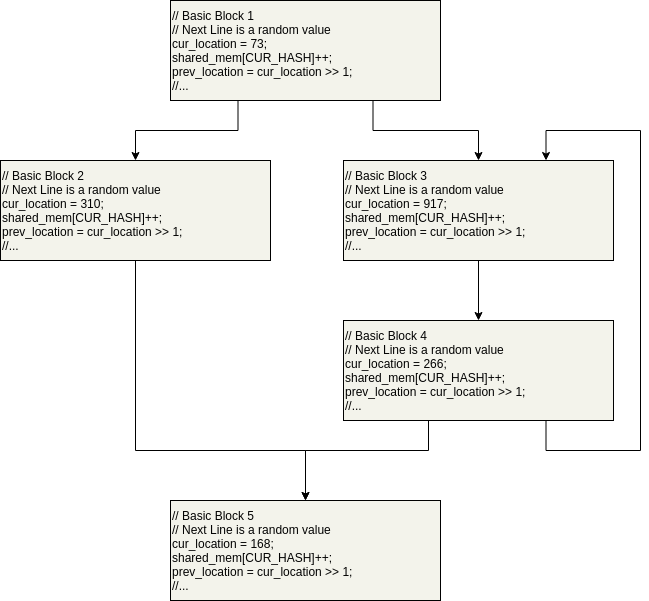
\includegraphics[width=\textwidth]{Chapter2/instrumentation.png}
    \centering
    \captionsetup{justification=centering}
    \caption{Example for instrumented basic blocks}
    \label{fig:instrumentation}
\end{figure}

AFL uses this coverage feature for discovering new inputs with new code coverages.

\subsubsection*{Visitor functions}

\say{Instruction visitors are used when you want to perform different actions for different kinds of instructions without having to use lots of casts and a big switch statement (in your code, that is). \cite{inst_visitor}} 

\lstinputlisting[language=C++,style=CodeStyle,label={lst:visitors},caption={Visitors example}]{Codes/Chapter2/visitor.cpp}

The specified range can be any two iterators, which can be a Module, Function, BasicBlock, Instruction or any other range between two instruction addresses.
